The evolution of digital systems described in the previous chapter provides the technological and conceptual context in which the Digital Twin paradigm has emerged. Increasing sensing capabilities, pervasive connectivity, distributed computing, and continuous data processing have made it possible to establish increasingly rich and persistent digital representations of physical entities and processes. Digital Twins build upon these capabilities by connecting physical systems with digital counterparts that can be used for monitoring, analysis, simulation, prediction, optimization, and decision support.

Despite the growing adoption of the term, however, Digital Twin remains a broad and heterogeneous concept. Different communities and application domains have proposed distinct definitions, architectures, and implementation approaches, often reflecting specific technological or operational requirements. This diversity has enabled the development of highly specialized solutions, but has also contributed to a fragmented landscape with limited interoperability between independently developed Digital Twin systems. As a result, the potential benefits of Digital Twins are often constrained by the difficulty of sharing and reusing information across different systems, applications, and domains.

This chapter examines the Digital Twin paradigm from this perspective. It first discusses the historical development of the concept and the heterogeneous interpretations that have emerged around its definition. It then examines reference architectures and the properties commonly associated with Digital Twins, highlighting the increasing complexity of the models, data, and computational capabilities involved. Building on this architectural discussion, it characterizes the data that Digital Twins produce and consume, and the requirements that follow from its unique characteristics. The discussion subsequently turns to the main challenges emerging from the proliferation of Digital Twin solutions. Finally, the chapter considers interoperability and standardization as emerging requirements for moving from isolated Digital Twin implementations towards interconnected Digital Twin ecosystems.

% =========================================================================

\section{History and Definition}
\label{sec:history-and-definition}
% =========================================================================
The Digital Twin concept origins are traced to Michael Grieves' work on Product Lifecycle Management (PLM)~\cite{grieves2014digital} at the beginning of the 2000s, where it was conceived as a virtual representation of a product throughout its lifecycle. The original conceptualisation introduced three fundamental components that characterize a DT, as also shown in \Cref{fig:grieves_dt}:
\begin{itemize}
    \item a \textit{physical space} and its products;
    \item a \textit{virtual space} with virtual representations of the products;
    \item a \textit{connection} between the two spaces, entailing an information flow between the two entities.
\end{itemize}

\begin{figure}[ht]
    \centering
    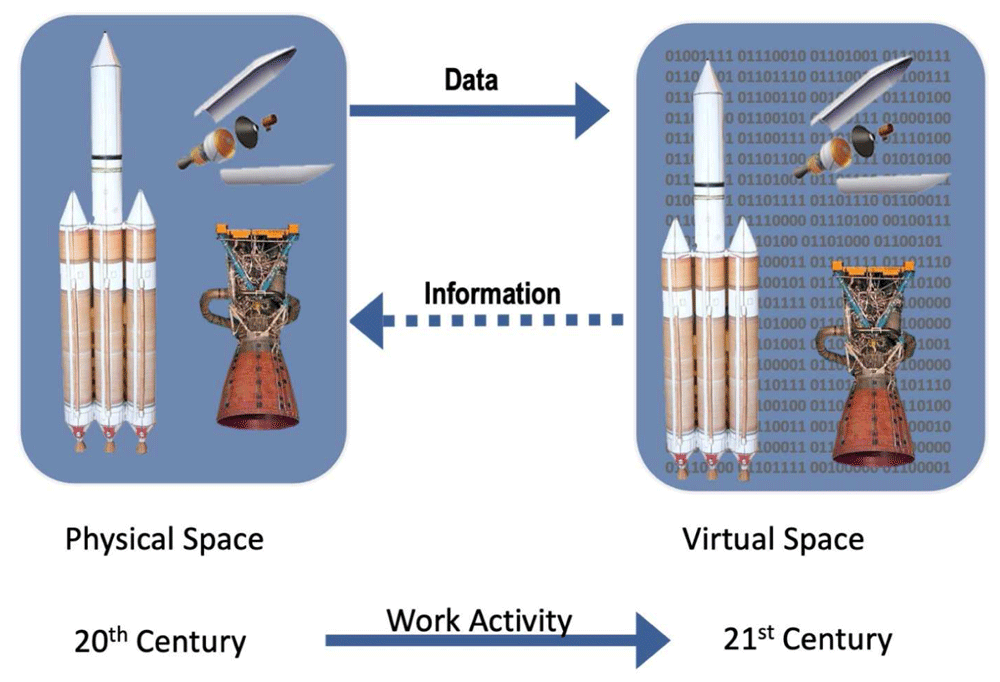
\includegraphics[width=0.65\textwidth]{parts/foundations/images/dt_model_grieves.png}
    \caption{The original DT conceptual model by Grieves, from~\cite{grieves2014digital}} 
    \label{fig:grieves_dt}
\end{figure}

Grieves' early-2000s work is generally regarded as the conceptual origin, while subsequent contributions associated the concept with the term \emph{Digital Twin} and extended it to aerospace and other engineering domains \cite{grieves2002,glaessgen2012,wuni2026}. 

This distinction is important because it places the relationship between the physical and digital spaces at the centre of the concept. The Digital Twin was conceived not merely as a model that could represent a physical object, but as a digital representation connected to it through an ongoing flow of information. In the original formulations, this connection enabled data describing the physical system to be incorporated into the virtual representation, while the information generated within the virtual space could be used to inform decisions concerning the physical system \cite{grieves2014digital,glaessgen2012}.

The subsequent diffusion of the concept was closely related to the development of Industry~4.0, the Internet of Things, industrial connectivity, and data analytics. As physical systems became increasingly instrumented and connected, the continuous acquisition of operational data made it possible to maintain increasingly dynamic digital representations. Digital Twins consequently moved beyond their original product-lifecycle-oriented formulation and were adopted across manufacturing, aerospace, energy, buildings, transportation, healthcare, smart cities, and other domains \cite{qi2021,liu2021,tao2022}.

The growth of the research field reflects this broad diffusion. Tao et al. reported more than 1,000 Digital Twin-related papers per year for three consecutive years beginning in 2019, with 2,934 papers published in 2021 \cite{tao2022}. More recent analyses show an even stronger increase. Wuni et al., analysing scientific and practitioner literature up to 2024, report a substantial growth in Digital Twin publications and identify the last decade as the period in which the vast majority of currently circulating definitions were introduced \cite{wuni2026}. The resulting literature is correspondingly broad, spanning multiple disciplines, application domains, technological approaches, and interpretations of the Digital Twin concept.

This rapid expansion has also created a conceptual problem. As the term has been adopted by communities with different backgrounds and objectives, Digital Twin has increasingly become an umbrella concept encompassing substantially different systems. Different studies may use the same term to describe a simulation model, a three-dimensional representation, a monitoring system, a predictive model, or a fully connected cyber-physical system. Several reviews have therefore identified the lack of a universally accepted definition as one of the persistent challenges of the field \cite{barricelli2019,jones2020,fuller2020,wuni2026}.

\begin{figure}[ht]
    \centering
    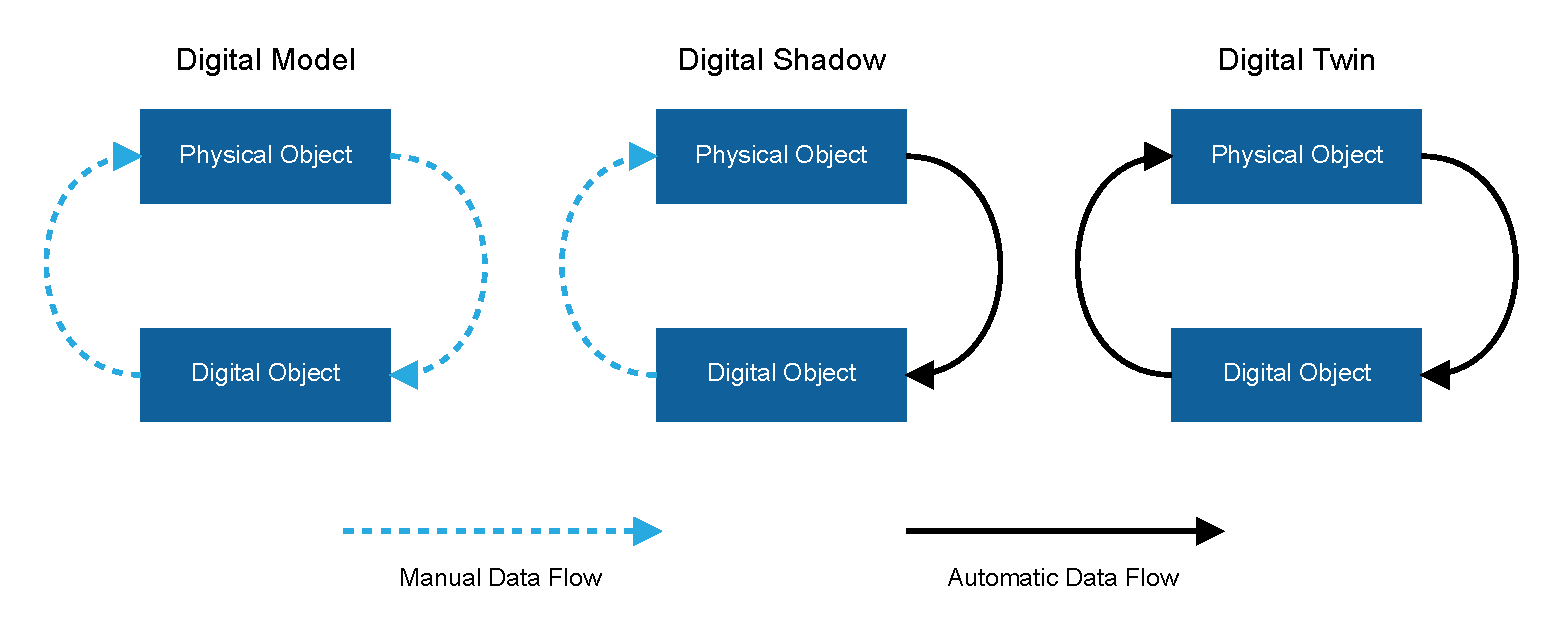
\includegraphics[scale=0.5]{parts/foundations/images/dmdsdt.pdf}
    \caption{Differences between Digital Model, Digital Shadow, and Digital Twin, adapted from Kritzinger et al.~\cite{kritzinger2018}.}
    \label{fig:dtdsdm}
\end{figure}

A particularly useful distinction in this context is the one between a \emph{Digital Model} (DM), a \emph{Digital Shadow} (DS), and a \emph{Digital Twin}, as shown in \Cref{fig:dtdsdm}. Kritzinger et al. introduced this distinction according to the degree and direction of information exchange between the physical and digital entities, a classification subsequently adopted by several reviews and studies \cite{kritzinger2018,fuller2020}. A DM represents a physical entity without an automated connection to it. Changes in the physical system therefore do not automatically propagate to the model, and changes in the model do not automatically affect the physical system.

A DS introduces an automated, but one-directional, connection. Information about changes occurring in the physical system is automatically transferred to the digital representation. The digital representation therefore provides an updated view of the physical system, but does not necessarily influence it automatically. A Digital Twin extends this relationship to bidirectional exchange: changes in the physical system can update the digital representation, while information or decisions generated in the digital space can affect the physical system \cite{kritzinger2018,fuller2020}.

The progression from DM to DT is not primarily determined by the complexity or fidelity of the digital representation, but by the nature and importance of the connection established between the physical and digital entities. A highly detailed three-dimensional simulation that is disconnected from its physical counterpart is therefore not necessarily a Digital Twin, while a less visually sophisticated representation may qualify as one if it is continuously connected to the physical system through an appropriate data flow.

The distinction also highlights the central role played by data in the Digital Twin concept. The transition from DM to DS is enabled by the introduction of an automated data flow, while the transition from DS to DT requires the ability to exchange information in both directions \cite{kritzinger2018,fuller2020}. Communication and data exchange are therefore not merely implementation details; they constitute one of the mechanisms through which the relationship between the physical and digital spaces is established.

Recent systematic analyses provide further evidence of the persistent difficulty of maintaining this conceptual distinction. Wuni et al. analysed 358 definitions from scientific and practitioner sources and found that 66.48\% captured the physical entity, its virtual counterpart, and a persistent bidirectional data and information flow, whereas 33.52\% described entities that, according to their classification, were more appropriately understood as Digital Models \cite{wuni2026}. The analysis also found that terms such as \emph{data}, \emph{information}, \emph{real-time}, \emph{representation}, and \emph{entity} are frequently present in Digital Twin definitions, while terms describing the continuous exchange itself are comparatively less represented \cite{wuni2026}.

This result is particularly relevant to the evolution of the concept. The literature has increasingly recognized that a Digital Twin cannot be reduced to a static representation. Nevertheless, the different formulations used to describe the connection, synchronization, and exchange between physical and virtual entities indicate that the data flow remains interpreted in substantially different ways across the literature. The conceptual core of the Digital Twin is therefore increasingly associated with continuity and synchronization, while the concrete mechanisms through which these properties are modelled and implemented remain strongly dependent on the application domain.

The definition of Digital Twin adopted in this thesis follows this core interpretation.

\begin{quote}
\textit{A Digital Twin is a digital representation of a physical entity or process, continuously connected to its physical counterpart through a bidirectional exchange of information. This enables the digital representation to stay updated with the physical state, while allowing insights generated in the digital space to trigger decisions and actions that directly affect the physical entity.}
\end{quote}

The digital representation may depend on multiple information sources, interact with other digital entities, and expose information that could be relevant to other applications. The more Digital Twins are deployed across interconnected domains, the more important the mechanisms governing their interaction become.

\section{Reference Architectures and Properties}
\label{sec:ref-arch}
% =========================================================================

The increasing adoption of Digital Twins has led to the development of several conceptual models and reference architectures intended to describe their main components and relationships. Although no single architectural representation has emerged as universally adopted, different proposals progressively extend the original conceptualization of the Digital Twin by introducing additional dimensions related to modelling, data, communication, and services \cite{qi2021,tao2022,liu2021}. These models provide useful abstractions for understanding how Digital Twins are structured and how their different components contribute to their operation.

The original formulation introduced by Grieves provided a deliberately simple conceptual representation based on three elements: a physical entity in the physical space, its virtual representation in the virtual space, and a connection enabling information exchange between the two \cite{grieves2014digital}. In this view, the virtual representation provides the digital counterpart of the physical entity, while the connection establishes the relationship through which information can be exchanged. The model therefore captures the fundamental physical--digital relationship underlying the Digital Twin concept.

As Digital Twin applications evolved beyond their original product-lifecycle context, more detailed architectural representations were proposed. One of the most widely referenced models is the five-dimensional Digital Twin model introduced by Tao et al., which extends the original three-part conceptualization by explicitly identifying five dimensions: \textit{physical entity}, \textit{virtual model}, \textit{connection}, \textit{data}, and \textit{service} \cite{tao2019,qi2021}. The model is illustrated in \Cref{fig:tao_dt}.

\begin{figure}[ht]
    \centering
    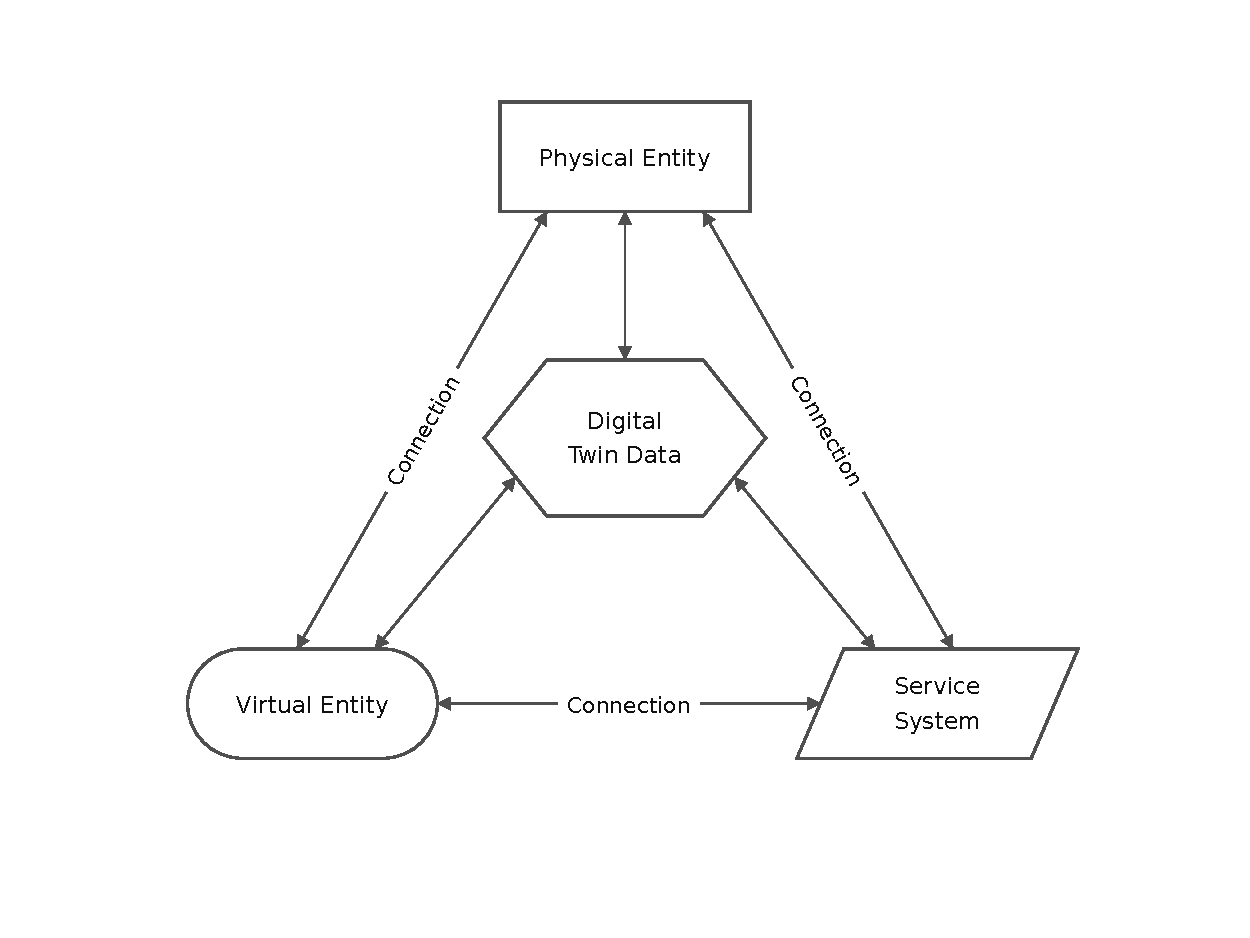
\includegraphics[scale=0.5]{parts/foundations/images/5dim_dt.pdf}
    \caption{Five-dimensional Digital Twin model, adapted from Tao et al.~\cite{tao2019,qi2021}.}
    \label{fig:tao_dt}
\end{figure}

The five-dimensional model provides a more comprehensive architectural view of a Digital Twin. The \textit{physical entity} represents the real-world object, system, or process being twinned, while the \textit{virtual model} provides its digital representation. The \textit{connection} establishes the communication between the physical and virtual spaces, enabling the exchange of information. The \textit{data} dimension captures the information generated, collected, and processed throughout the operation of the Twin, while \textit{services} represent the functionalities offered through the Digital Twin.

Within this model, the virtual representation is not necessarily limited to a single type of model. Tao et al. distinguish geometric, physical, behavioural, and rule models as complementary dimensions that can be combined to represent different aspects of the physical entity \cite{tao2022}. Geometric models describe the shape and structural characteristics of an entity; physical models capture relevant physical properties and constraints; behavioural models describe its dynamic evolution; and rule models incorporate rules, historical information, and domain knowledge. Depending on the application, these models can support simulation, prediction, optimization, diagnosis, and other computational functions.

The explicit introduction of data as a separate dimension, and specifically placed at the core of the architecture,  is particularly relevant to the evolution of Digital Twins. In the original three-component formulation, data was implicitly associated with the connection between the physical and virtual spaces. In the five-dimensional model, it is instead represented as an independent and pivotal architectural element connecting the physical entity, virtual model, connection, and services \cite{qi2021,tao2022}.

Data is therefore involved throughout the operation of a Digital Twin. Measurements and observations produced by the physical entity can be collected and used to update its virtual representation. Historical information can complement current observations, while data-driven and model-based techniques can transform these inputs into higher-level information and knowledge. The resulting outputs can support services such as monitoring, simulation, prediction, optimization, and decision making \cite{qi2021,tao2022}. Finally, outputs produced within the virtual reèresentation can in turn be used to determine actions affecting the physical entity.

As shown in numerous research articles, the diversity of application domains has consequently resulted in a wide range of Digital Twin architectures and implementations. Tao et al. reviewed 284 publications on Digital Twin models and found that almost half concerned manufacturing applications. Energy represented 35 publications and aerospace 20, while further applications were identified in areas such as engineering construction, cities, healthcare, transportation, and environmental systems \cite{tao2022}. This distribution illustrates the progressive diffusion of the concept from its initial engineering and manufacturing context towards a much broader set of application domains.

Architectural variation also emerges from the scale of the physical systems being represented. Tao et al. distinguish between unit-level, system-level, and System-of-Systems (SoS)-level Digital Twin models \cite{tao2022}. At the unit level, a Twin may represent an individual component or piece of equipment. At the system level, it may represent a production line, aircraft subsystem, building, or other integrated system composed of multiple components. At the SoS level, the Digital Twin represents a collection of interacting systems whose behaviour depends on the relationships between their constituent parts.

This hierarchical perspective is particularly relevant to the architecture of complex Digital Twin Environments (DTE).
%
The concept of DTE traces back to Grieves~\cite{Grtz2026}, who envisioned aggregating homogeneous DT instances to observe population-level behaviors and trends across identical products. In contrast, the modern framing of a Digital Twin Ecosystem (DTE) is largely shaped by the UK's National Digital Twin programme.
%
Under this paradigm, the National Digital Twin is defined as “an ecosystem of digital twins and the protocols by which they can be integrated securely and resiliently”~\cite{dtarch}. 
%
A Digital Twin at one level may therefore coexist with other Twins representing related entities at different levels of abstraction. In a manufacturing environment, for example, individual machines may be represented by dedicated Digital Twins, while a production line may be represented at a higher level by a Twin that considers the interactions among those machines. Similar hierarchical relationships can be found in other domains, such as aerospace, healthcare, and urban systems \cite{tao2022}.

Recent reference architectures have increasingly conceptualized the Digital Twin not as a tailored, self-contained entity, but as a modular platform component governed by service-oriented principles. Aligning with this perspective, Aheleroff et al. \cite{AHELEROFF2021101225} proposed a \emph{Digital Twin as a Service} (DTaaS) reference model for Industry 4.0. Their work highlights the necessity of abstracting DT functionalities into scalable, cloud-based services to support complex system integration across a large number of assets. Crucially, this DTaaS approach acts as an architectural blueprint: rather than dictating a monolithic structure, it identifies the mandatory infrastructural modules required to operate a DT. By standardizing these core components into composable building blocks, the architecture empowers developers to flexibly assemble, instantiate, and scale customized Digital Twins. Consequently, the development focus shifts from engineering isolated systems from scratch to leveraging a shared, service-oriented infrastructure that inherently fosters standardization and interoperability.

Across these different approaches, the specific technologies and internal structures may vary considerably, but several architectural elements recur: a physical entity, a digital representation, mechanisms for exchanging information between the two, data supporting the representation and its operation, and services built on top of the available models and information. The balance among these elements depends strongly on the domain, the characteristics of the physical system, and the intended functionality of the Digital Twin.

The literature therefore presents the Digital Twin not as a single architectural pattern, but as a family of related architectural abstractions. The original three-component model provides a conceptual foundation centered on the physical--digital relationship, while subsequent models introduce additional dimensions to capture the data, models, and services required by increasingly sophisticated implementations. In particular, the explicit introduction of data as an architectural dimension represents an important step in the evolution of the concept, reflecting the increasing role of information in maintaining, operating, and exploiting Digital Twins. Having recurred, in every reference architecture discussed above, as the element connecting the physical entity, its virtual representation, and the services built on top of it, data deserves to be examined in its own terms as the basis for the data-oriented perspective developed in the remainder of this thesis.

\section{Challenges and Opportunities}

\label{sec:challenges}

The increasing adoption of Digital Twins across different application domains introduces significant opportunities for monitoring, analysis, simulation, optimization, and decision support. At the same time, the current state of development of Digital Twins presents several challenges related to their increasing \textit{complexity} and wide \textit{heterogeneity}. In terms of heterogeneity, DTs may differ with respect to the physical systems they represent, the goals they pursue, the data they rely on, and most notably, the technologies and architectures used for their implementation.
%
Some of these differences are the result of the limited degree of \textit{standardization} achieved so far, despite the research community having strongly advocated for greater standardization efforts over the last decade \cite{wang2022standards,wuni2026}.
%
While the number of publications related to DTs has increased extremely rapidly, the literature shows that some studies still fail to provide a clear definition of the DT concept and consequently, at least partially, fail to reflect its essential characteristics in their implementations. Others provide definitions that are not consistent with one another \cite{wuni2026,tao2022}.
%
The lack of standardization also hinders the development of frameworks, reference architectures, and platforms capable of supporting the development of DTs in a consistent and modular way.
%
Furthermore, if standardization is already a challenge within individual DTs, its absence becomes even more relevant when considering more complex scenarios such as DTEs, in which multiple DTs are expected to coexist and meaningfully interact.

The meaningful interaction required within DTEs introduces a further challenge related to \textit{interoperability}. Independently developed DTs need to be able to communicate and exchange information in a way that is meaningful for all the systems involved. This requires not only a technical connection between the systems, but also a shared understanding of the exchanged information, including its semantics and context. Interoperability is therefore a multi-level challenge encompassing technical, syntactic, and semantic aspects, and requiring mechanisms to manage differences between independently developed systems.

Heterogeneity and the resulting lack of coordination between independently developed Digital Twins are, in this sense, the root of the problem. Addressing them requires progress along two related fronts. \textbf{Standardization} is the primary lever available for this purpose: the definition of common principles, structures, and mechanisms that can provide shared foundations for developing and managing Digital Twins, thereby reducing unnecessary heterogeneity. \textbf{Interoperability} is the capability such foundations are meant to enable: the ability of different, independently developed Digital Twins to communicate, exchange information, and cooperate effectively. Standardization and interoperability are therefore closely related (the former is typically a precondition for the latter) but they address different aspects of the problem and, as discussed below, are not always achieved together.
%
These two dimensions will be discussed from two different perspectives: single Digital Twins and Digital Twin Ecosystems. The former primarily concerns the development of individual Digital Twins, while the latter concerns the interaction between multiple independently developed Digital Twins.

\subsection{Standardization}

At the level of an individual Digital Twin, standardization can provide a common foundation for its construction and management. Rather than defining every Digital Twin as a completely independent solution, standardized building blocks, architectural principles, and mechanisms can guide developers in assembling the components required by a particular application. Such standardization does not require all Digital Twins to have the same structure or capabilities. Instead, it can provide a common set of elements from which different Digital Twins can be constructed and tailored to their specific requirements.

At the level of a Digital Twin Ecosystem (DTE), the scope of standardization becomes broader. A DTE involves multiple Digital Twins that may have been developed independently and may rely on different technological solutions. Standardization can therefore concern the common foundations of the ecosystem itself, including the infrastructure, architectural principles, interfaces, and data representations that support the deployment and interaction of multiple Digital Twins. In this sense, standardization can reduce unnecessary differences between implementations and provide a common basis on which heterogeneous Digital Twins can coexist.

Wang et al. review the landscape of Digital Twin standardization efforts, consolidating contributions from organizations including the International Organization for Standardization (ISO), the International Electrotechnical Commission (IEC), the International Telecommunication Union (ITU), and the Institute of Electrical and Electronics Engineers (IEEE) \cite{wang2022standards}. Their review is framed around the five-dimensional Digital Twin model introduced by Tao et al., comprising the physical entity, virtual model, connection, data, and services \cite{tao2019,qi2021}. For the purposes of this thesis, two of these dimensions are particularly relevant: the \textit{connection}, which provides the infrastructural basis for communication and interaction, and \textit{data}, which constitutes the information exchanged and processed by the different components of the Digital Twin.

From an infrastructural perspective, standardization addresses the mechanisms through which Digital Twins and their components can connect and communicate. Common interfaces, communication protocols, service descriptions, and architectural principles can reduce implementation-specific dependencies and facilitate the integration of independently developed components. Wang et al. identify the lack of common references for Digital Twin architectures and communication mechanisms as an important obstacle to the interconnection of Digital Twin components and services across different systems and domains \cite{wang2022standards}. Standardization at this level therefore provides the technical foundations required for Digital Twin systems to communicate.

A second and complementary dimension concerns the data exchanged through these infrastructures. Digital Twins continuously produce, consume, and transform information originating from physical entities, models, sensors, information systems, and other computational services. Wang et al. identify several standardization requirements related to Digital Twin data, including the processing of heterogeneous data, the management of multi-source and multi-modal data, and mechanisms concerning data syntax, semantic mapping, and data exchange \cite{wang2022standards}. These requirements indicate that standardization cannot be limited to the mechanisms used to transport data; the representation and interpretation of the exchanged information are equally, if not more so, relevant.

These two dimensions of standardization, of the infrastructure used to connect Digital Twins, and of the data they exchange, do not exhibit the same degree of maturity. Communication and interface standards provide increasingly established mechanisms through which heterogeneous systems can connect, while data-oriented standards and semantic approaches are comparatively less developed \cite{wang2022standards}. This gap becomes especially relevant within a Digital Twin Ecosystem: while an individual Digital Twin can often rely on tightly coupled, internally consistent interfaces and data representations, a Digital Twin Ecosystem brings together systems designed around different assumptions, so that establishing a communication channel between them is only a first step. Standardizing that channel does not, by itself, guarantee that the information exchanged through it will be correctly interpreted by the receiving system.

From this perspective, standardization should not be understood as an attempt to impose a single implementation on all Digital Twins. Domain-specific models, technologies, and services may remain necessary to address the characteristics of individual physical systems. The objective is instead to identify and standardize the common elements at the boundaries between systems, allowing Digital Twins to retain their internal specialization while remaining capable of participating in a broader ecosystem. Achieving such common foundations can reduce the effort required to develop new Digital Twins, facilitate their integration, and enable the reuse of data and services across applications. It can also support the development of reusable frameworks and platforms capable of deploying and managing Digital Twins according to shared architectural principles.     However, providing common foundations does not, by itself, guarantee that independently developed Digital Twins can effectively work together. This motivates the following discussion, which considers interoperability as a distinct challenge in its own right.

\subsection{Interoperability}

Interoperability becomes particularly relevant at the level of the Digital Twin Ecosystem. When multiple Digital Twins are independently developed, they may rely on different architectures, interfaces, data representations, and terminology. The challenge is therefore to enable these systems to communicate seamlessly and to exchange information that can be correctly understood and used by the receiving system.

At the level of an individual Digital Twin, there is no interoperability problem in the sense of interaction between independently developed Digital Twins, since the system is considered in isolation. Internal components still need to interact with one another, but this is primarily a matter of designing and integrating the Digital Twin itself. Interoperability becomes a distinct concern when multiple Digital Twins are brought together within a DTE.

This distinction is important because interoperability does not simply mean connecting systems despite their differences. Rather, it concerns finding ways to integrate those differences so that independently developed systems can communicate and make meaningful use of the information exchanged between them. A system should not merely receive a message from another system; it should be able to understand what that information represents and use it within its own context.

This requirement becomes particularly important when Digital Twins exchange information that contributes to monitoring, analysis, or decision-making. Two systems may use different representations for the same physical phenomenon, and a successful interaction requires more than a technical connection between them. The receiving system must be able to interpret the exchanged information according to its intended meaning and context.

Recent literature has begun to characterize this problem more precisely, distinguishing between several levels at which interoperability between Digital Twins can be assessed and pursued. Acharya et al.~\cite{acharya2024interoperability}, surveying interoperability within Digital Twin deployments in cyber-physical systems, delineate distinct interoperability levels and examinTheir analysis proposes a framework of six such levels -- \textit{technical}, \textit{syntactic}, \textit{semantic}, \textit{pragmatic}, \textit{dynamic}, and \textit{organizational} -- ranging from the basic ability of Digital Twins to exchange messages over a common communication infrastructure, through agreement on a common structure and encoding for the exchanged data, up to the higher-level ability to agree on the meaning of the exchanged concepts and on the business or operational context in which they are used. For the purposes of this thesis, the technical, syntactic, and semantic levels are the most directly relevant, since they map most closely onto the software/data distinction followed here.
%
David et al. similarly review the challenges affecting interoperability among Digital Twins, together with the factors that have been found to contribute to successful interoperable deployments, and outline directions for future research on the topic \cite{david2024interoperability}. Both contributions confirm that achieving interoperability across independently developed Digital Twins requires more than establishing a technical connection between them.

A simple example makes the semantic level concrete: two Digital Twins monitoring similar physical processes may represent the same measured quantity, such as temperature, under different property names, units, or data structures. A compatible communication channel is sufficient to transmit the corresponding value from one system to the other, but it does not by itself guarantee that the receiving system correctly identifies what that value represents; establishing this correspondence is a matter of semantic, rather than merely technical or syntactic, interoperability.

Standardization and interoperability therefore address complementary aspects of the same underlying problem: the former provides shared architectural and data-related foundations for constructing Digital Twins and Digital Twin Ecosystems, while the latter concerns the ability of independently developed Digital Twins to exchange and meaningfully reuse each other's information once such foundations are in place. The following chapter examines this problem from the perspective of the data involved, characterizing the data that Digital Twins produce and consume and the mechanisms required to manage it consistently across independently developed systems.